\chapter{Fluid Kinematics}
This chapter is based on Munson Chapter 4.

\section{The Velocity Field}

There are two ways of describing a fluid flow, the Eularian, and the Lagrangian approach:
\subsection{Difference Between Eularian and Lagrangian Approach}
For the Eularian approach, we define a velocity field which is a function of the three-dimensional position $\vec r$ and time $t$. From this we know where at which time the stream lines point in a certain direction.

The Lagrangian approach follows particles: A large amount of particles are released and traced as a function of time. 

\begin{figure}[H]
	\centering
	\begin{subfigure}{0.45\textwidth}
		\centering
		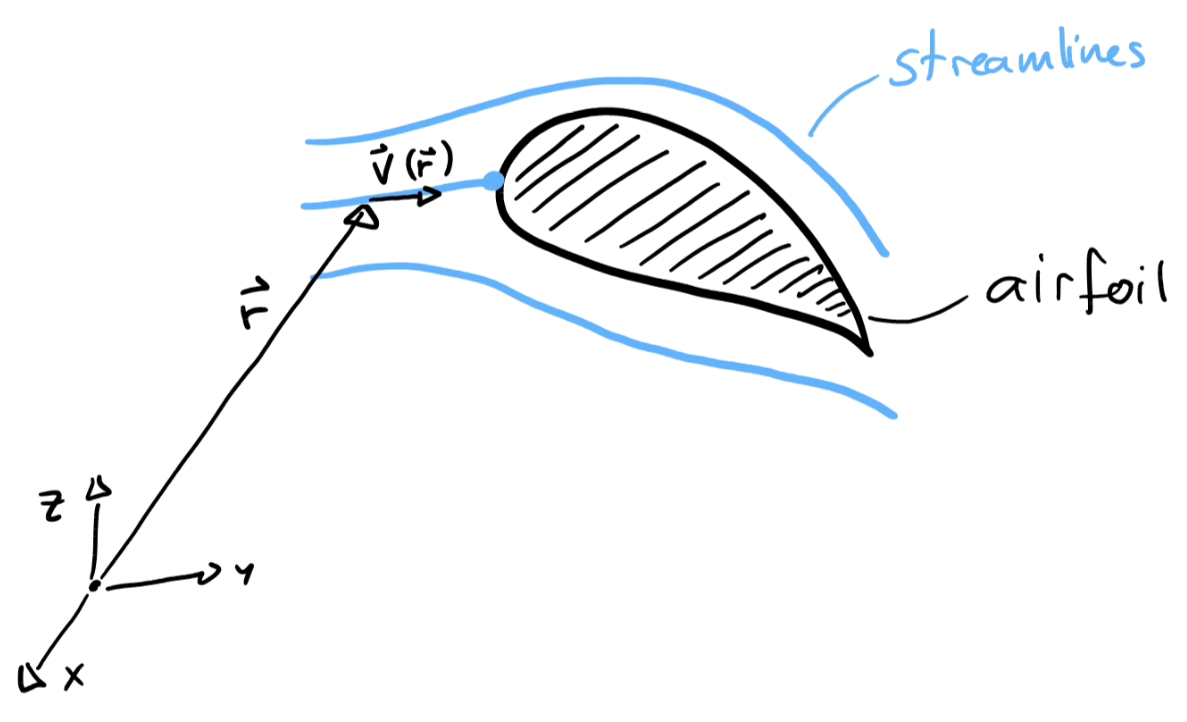
\includegraphics[width=\linewidth]{Sketches/EularianVelocityField}
		\begin{equation*}
			\vec V ( \vec r,t)
		\end{equation*}
		\caption{Eulerian velocity field}
		\label{fig:eularianvelocityfield}
	\end{subfigure}%
	\hfill
	\begin{subfigure}{0.45\textwidth}
		\centering
		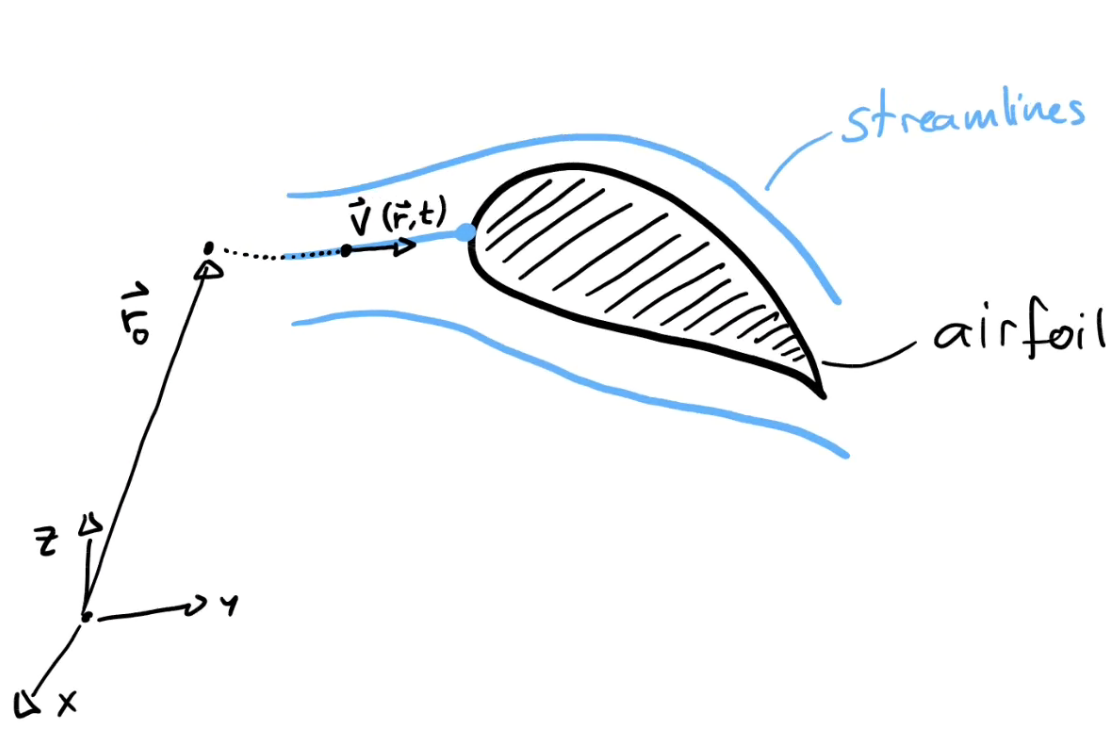
\includegraphics[width=\linewidth]{Sketches/LagrangianVelocityField}
		\begin{equation*}
			\vec V(\vec r_0,t)
		\end{equation*}
		\caption{Lagrangian velocity field}
		\label{fig:lagrangianvelocityfield}
	\end{subfigure}
	\caption{Comparison of (a) Eulerian and (b) Lagrangian velocity field representations}
	\label{fig:velocity_fields}
\end{figure}

\subsection{Visualizing Flows}
\begin{itemize}
	\item \textbf{Stream Line} (\textit{SL}) A line tangent to the velocity vector at any point.

	\begin{figure}[H]
			\centering
			\raisebox{-.5\height}{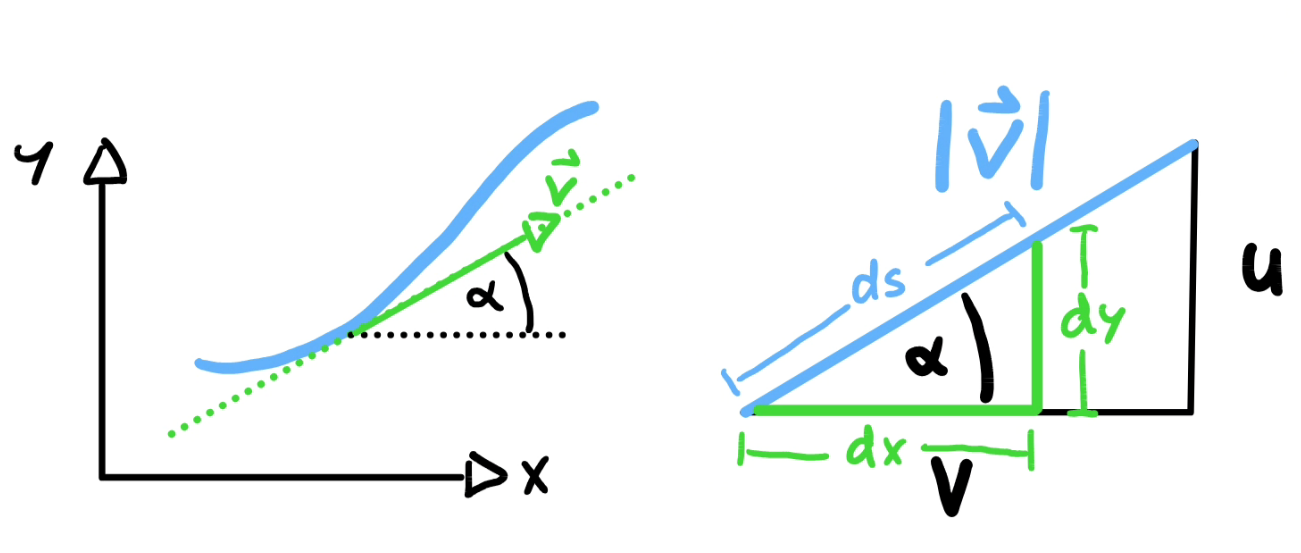
\includegraphics[width=0.4\linewidth]{Sketches/StreamLineEquationDerivation}}
			\label{fig:streamlineequationderivation}
	\end{figure}
	
	\begin{equation*}
		\boxed{\frac{dy}{dx} = \frac vu\qquad \frac{dz}{dx} = \frac wu \qquad \frac{dz}{dy} = \frac wv}
	\end{equation*}
	
	we can define the parametrised curve $\vec r_{sl}(s)$, described by:
	\begin{equation*}
		\frac{d\vec r_{sl}(s)}{ds} \times \vec V (\vec r_sp) = \vec 0
	\end{equation*}
	Stream lines are a purely Eurlarian concept.
	
	\item \textbf{Path Line} Line describing the actual path of a fluid element.

	\begin{equation*}
		\frac{d\vec r_p}{dt} = \vec V (\vec r_p(t))
	\end{equation*}
	where $V$ is the velocity at the instantaneous particle location and $\vec r_p$ is the position of a particle. In components this will result in:
	\begin{equation*}
		\boxed{\frac{dx}{dt} = u\qquad \frac{dy}{dt} =v\qquad \frac{dz}{dt} = w}
	\end{equation*}
	This is meant in a Lagrangian sense: We track a particle and register its position as a function of time.
	
	Similarly, we could write, as a ordinary differential equation:
	\begin{equation*}
		\frac{d\vec r_{pl}}{d t} = \vec V(\vec r_{pl},t)\qquad \text{where } \vec r_{pl} (t=t_0) = \vec r_{p_0}
	\end{equation*}
	
	
	\item \textbf{Steak Line} A line made up of particles, that have previously passed through a common point. It can be reconstructed from path lines: 
	\begin{equation*}
		\frac{d \vec \tau_p}{dt} = V(r_p,t)\qquad\text{width }\vec r_p(t=\tau_p) = \vec r_0\implies \vec r_p (t,\tau_p)
	\end{equation*}
\end{itemize}




\begin{figure}[H]
	\centering
	\begin{subfigure}{0.3\textwidth}	
		\centering
		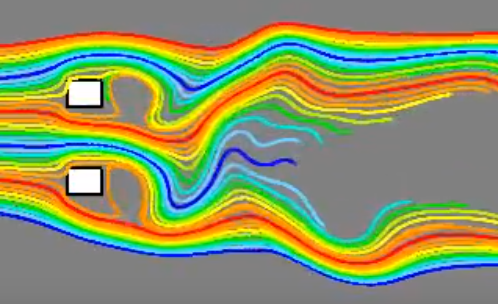
\includegraphics[width=\linewidth]{Sketches/StreamLine}
		\caption{Stream Line}
		\label{fig:streamlines}
	\end{subfigure}
	\hfill
	\begin{subfigure}{0.3\textwidth}
		\centering
		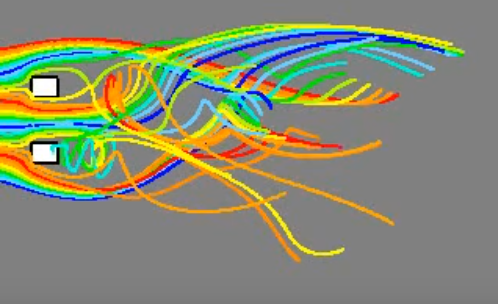
\includegraphics[width=\linewidth]{Sketches/PathLine}
		\caption{Path Line}
		\label{fig:pathline}
	\end{subfigure}%
	\hfill
	\begin{subfigure}{0.3\textwidth}
		\centering
		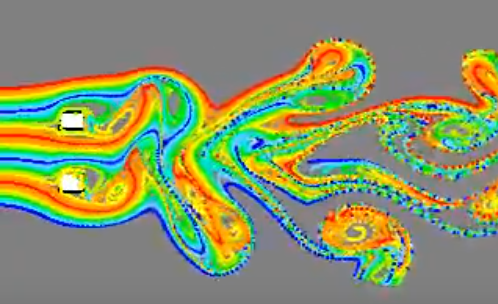
\includegraphics[width=\linewidth]{Sketches/StreakLine}
		\caption{Streak Line}
		\label{fig:streakline}
	\end{subfigure}
	\caption{Comparison of stream, path, and streak line.}
\end{figure}

\subsubsection{Observation}
\begin{center}
	\shadowbox{If the flow is steady, then stream, path and streak lines are identical.}
\end{center}

\subsubsection{Example: Sprinkler (Munson 4.3)}

\begin{figure}[H]
	\centering
	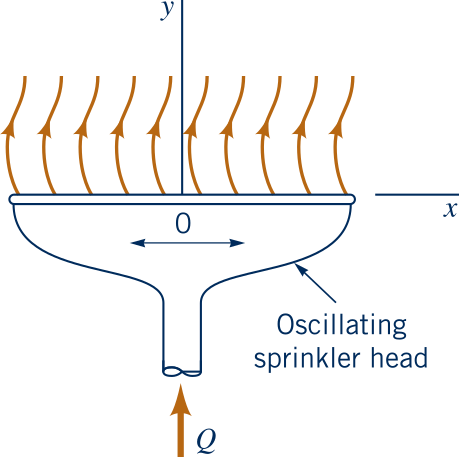
\includegraphics[width=0.45\linewidth]{Sketches/Sprinkler}
	\label{fig:sprinkler}
\end{figure}

let $\omega$ be the oscillation frequency, assume that $x$ and $y$ are infinitely extended. We are given the Eularian velocity field:
\begin{equation*}
	\vec V = U_0\sin\left(\omega \left( t - \frac {y}{v_0}\right)\right)\hat i + v_0 \hat j
\end{equation*}

\paragraph{Stream Line}
From the equation for streamlines we know:
\begin{equation*}
	\begin{split}
		\frac{dy}{dx} &= \frac vu  =\frac{v_0}{U_0\sin\left(\omega \left( t - \frac {y}{v_0}\right)\right)}\\
		U_0 \sin\left(\omega \left( t - \frac {y}{v_0}\right)\right) \,dy & =v_0 \,dx\\
		\int U_0 \sin\left(\omega \left( t - \frac {y}{v_0}\right)\right) \,dy & =\int v_0 \,dx\\ 
		U_0\frac{v_0}{\omega}\cos\left(\omega \left( t - \frac {y}{v_0}\right)\right) & =v_0x + C\\
		\implies x(y) &= \frac{u_0}{\omega}\cos\left(\omega \left( t - \frac {y}{v_0}\right)\right) + C'
	\end{split}
\end{equation*}
We want the stream lines to pass through the origin at $t_0=0$, therefore $C' = \frac {u_0}\omega$:
\begin{equation*}
	x = \frac {u_0}{\omega}\left(\cos\left(\frac{y\omega}{v_0}\right)-1\right)
\end{equation*}
\begin{figure}[H]
	\centering
	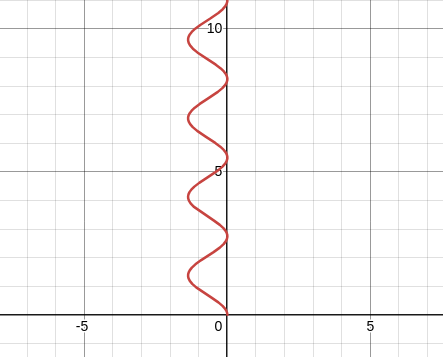
\includegraphics[width=0.4\linewidth]{Sketches/SprinklerStreamLine}
	\caption{Plot of $x(y)$ with $u_0=1.1, \omega= 1.6, v_0=0.7$}
	\label{fig:sprinklerstreamline}
\end{figure}


\paragraph{Path Line}
From the equations of the path line\footnote{in the Lagrangian sense, therefore $y=y(t)$ is the particles position instead of the initial position}, we know:
\begin{equation*}
	\frac{dx}{dt} = U_0 \sin\left(\omega \left( t - \frac {y(t)}{v_0}\right)\right)\qquad \frac{dy}{dt} = v_0
\end{equation*}
We first solve the differential equation for the $y$, yielding:
\begin{equation*}
	y(t) = v_0 t+ c_1
\end{equation*}
plugging this in, we transform the first differential equation into
\begin{equation*}
	\frac{dx}{dt} = U_0 \sin\left(\omega \left( t - \frac {v_0t + c_1}{v_0}\right)\right)=-U_0 \sin\left(\frac {\omega c_1}{v_0}\right)
\end{equation*}
The right hand side are all constants, therefore we can trivially find the solution for $x$:
\begin{equation*}
	x = -U_0\sin\left(\frac{c_1 \omega}{v_0}\right) t + c_2
\end{equation*}

Our parametric equations for path lines are
\begin{equation*}
	\begin{cases}
		x(t) = -U_0\sin\left(\frac{c_1 \omega}{v_0}\right) t + c_2\\
		y(t) = v_0 t+ c_1
	\end{cases}
\end{equation*}
We can represent different particles by varying $c_1$ and $c_2$. For example through algebra, we can find the constants of the particle that is released at $t=0$ at the origin $(x,y)=\vec 0$ to be $c_1=0, c_2=0$.
The path line of this particle is given by:
\begin{equation*}
	\begin{cases}
		x(t) = 0\\
		y(t) = v_0 t
	\end{cases}
\end{equation*}
meaning that it will move along the $y$ axis.


\paragraph{Streak Line}
We choose the streak line that goes though the origin at $t=0$. Knowing that streak lines can be reconstructed from path lines, we try to list all streak lines possible. They will all be linear with slopes varying from $\pm v_0/u_0$. As a streak line we will get something like the following picture:
\begin{figure}[H]
	\centering
	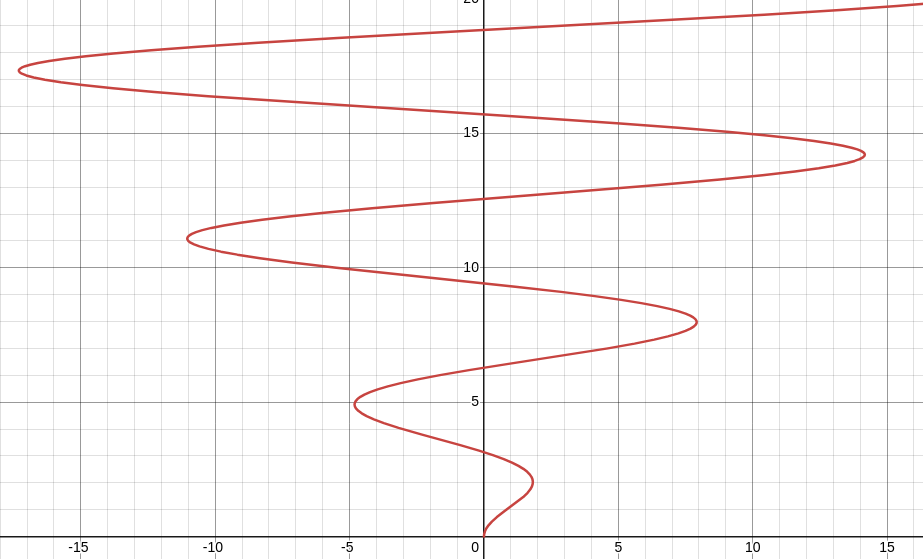
\includegraphics[width=0.4\linewidth]{Sketches/SprinklerStreakLine}
	\label{fig:sprinklerstreakline}
\end{figure}
Which is exactly what we would observe as a bystander.






